\documentclass[12pt, a4paper, oneside, UTF8]{ctexart}
\usepackage{amsmath, amsthm, amssymb, bm, color, framed, graphicx, hyperref, mathrsfs}
\usepackage{geometry}
\usepackage{caption}
\geometry{left = 2.5 cm, right = 2.5 cm, top = 2.5 cm, bottom = 2.5 cm}

\title{\textbf{作业12}\\{\small (数值算法与案例分析)}}
\author{李维杰}
\date{\today}
\linespread{1.5}
\definecolor{shadecolor}{RGB}{241, 241, 255}
\newcounter{problemname}
\newenvironment{problem}{\begin{shaded}\stepcounter{problemname}\par\noindent\textbf{题目\arabic{problemname}. }}{\end{shaded}\par}
\newenvironment{solution}{\par\noindent\textbf{解答. }}{\par}
\newenvironment{note}{\par\noindent\textbf{注记. }}{\par}

\newcommand{\pll}{\kern 0.56em/\kern -0.8em /\kern 0.56em}

\begin{document}

\maketitle

\begin{problem}
    实现GMRES算法,并用至少两个包含1000+个未知数的稀疏线性方程组(对称的和非对称的)测试,绘制残差的变化历程.
\end{problem}

\begin{solution}
    (代码见Problem1.m)
    \begin{figure}[htbp]
        \centering
        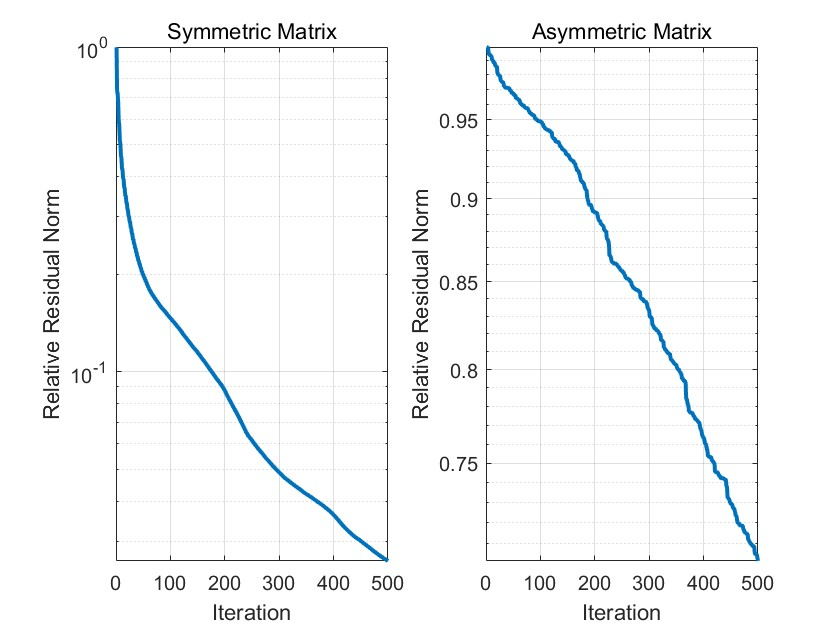
\includegraphics[scale=0.5]{Problem1.jpg}
        \caption{GMRES算法分别作用于包含$1000$个未知数的两种类型线性方程组的表现}
    \end{figure}
\end{solution}

\begin{problem}
    给定对称正定阵$A \in \mathbb{R}^{n \times n}$. 设$r_k$是SD算法解$Ax=b$时的第$k$步迭代时的残差向量. 
    证明:当$r_{k+1}=0$时,$r_k$是$A$的一个特征向量.
\end{problem}

\begin{solution}
    根据SD法的迭代步骤,有$x_{k+1} = x_{k} + \frac{r_k^T r_k}{r_k^T A r_k} r_k$.则当$r_{k+1} = 0$时,我们有
    $$Ax_k + A \frac{r_k^T r_k}{r_k^T A r_k} r_k - b = 0,$$
    即
    $$r_k = A \frac{r_k^T r_k}{r_k^T A r_k} r_k \Rightarrow A r_k = \frac{r_k^T A r_k}{r_k^T r_k} r_k.$$
\end{solution}

\begin{problem}
    给定对称正定阵$A \in \mathbb{R}^{n \times n}$.设$x_k$是SD算法解$Ax=b$时的第$k$步迭代时的近似答案. 
    证明:$$f(x_{k+1}) \leq (1 - {\kappa}^{-1})f(x_k),$$其中$f(x) = x^T A x - 2b^T x$并且$\kappa = {\left\lVert{A}\right\rVert}_{2}{\left\lVert{A^{-1}}\right\rVert}_{2}$.
\end{problem}

\begin{solution}
    由于
    \begin{align*}
        f(x_k) - f(x_{k+1}) &= \left\langle x_k, x_k \right\rangle _A - 2 \left\langle b, x_k \right\rangle - \left\langle x_k + \alpha_k r_k, x_k + \alpha_k r_k \right\rangle _A + 2 \left\langle b, x_k + \alpha_k r_k \right\rangle  \\
        &= -2 \alpha_k \left\langle x_k, r_k \right\rangle _A + 2 \alpha_k \left\langle b, r_k \right\rangle - {\alpha_k}^2 \left\langle r_k, r_k \right\rangle _A \\
        &= \frac{(r_k^T r_k)^2}{r_k ^T A r_k},
    \end{align*}
    又由于$A^{-1}$也是对称正定的,故
    \begin{align*}
        f(x_k) &= \left\langle x_k, x_k \right\rangle _A - 2\left\langle b, x_k \right\rangle \\
        &= \left\langle A^{-1}(b-r_k), A^{-1}(b-r_k) \right\rangle _A - 2\left\langle b, A^{-1}(b-r_k) \right\rangle \\
        &= r_k^T A^{-1} r_k - b^T A^{-1} b \\
        &\leq r_k^T A^{-1} r_k.
    \end{align*}
    则证明$f(x_{k+1}) \leq (1 - {\kappa}^{-1})f(x_k)$,等价于$\kappa \geq \frac{f(x_k)}{f(x_k) - f(x_{k+1})}$,即只需证
    \begin{align*}
        \frac{r_k^T A^{-1} r_k}{r_k^T r_k} \frac{r_k^T A r_k}{r_k^T r_k} \leq \kappa = (\frac{\lambda_n(A^2)}{\lambda_1(A^2)})^{1/2}.
    \end{align*}
    事实上由Rayleigh-Ritz定理,我们有
    \begin{align*}
        \max{\frac{r_k^T A^{-1} r_k}{r_k^T r_k}} &= \lambda_n(A^{-1}) = \frac{1}{\lambda_1(A)} \\
        \max{\frac{r_k^T A r_k}{r_k^T r_k}} &= \lambda_n(A)
    \end{align*}
    于是
    \begin{align*}
        \frac{r_k^T A^{-1} r_k}{r_k^T r_k} \frac{r_k^T A r_k}{r_k^T r_k} \leq \frac{\lambda_n(A)}{\lambda_1(A)} = (\frac{\lambda_n(A^2)}{\lambda_1(A^2)})^{1/2}.
    \end{align*}
\end{solution}

\begin{problem}
    使用SD算法解线性方程组$$\left[
        \begin{array}{cc}	
            20 &   \\
               & 1 \\
        \end{array}
    \right] x = 0,$$
    实现时,以$x_0 = [1, 5]^T$为初始假设, 并绘制中间近似值$x_k(0 \leq k \leq 10)$.
\end{problem}

\begin{solution}
    (代码见Problem4.m)
    \begin{figure}[htbp]
        \centering
        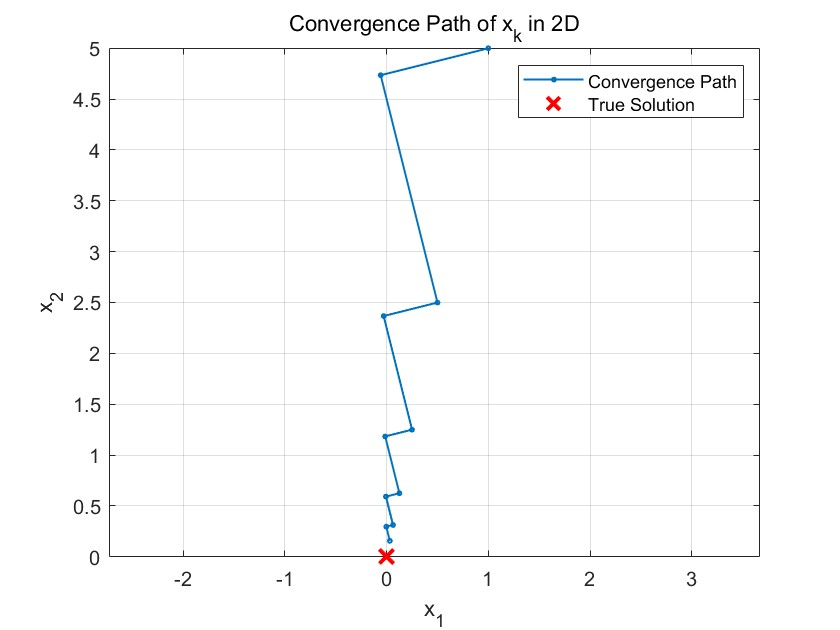
\includegraphics[scale=0.5]{Problem4.jpg}
        \caption{中间近似值$x_k(0 \leq k \leq 10)$}
    \end{figure}
\end{solution}
\end{document}